\documentclass[10pt]{standalone}
\usepackage{tikz}
\usetikzlibrary{backgrounds,calc,positioning}

\newcommand{\sh}{0.8cm}
\newcommand{\mh}{2.3cm}

\tikzset{
    lblock/.style = {
        draw, fill=blue!20, rectangle, align=center,
        outer sep=0,
        inner sep=0,
        minimum width={width("PC")+2pt},
        minimum height={width("RegisterMapper")*2},
        font=\small
    },
    mblock/.style = {
        draw, fill=blue!20, rectangle, align=center,
        outer sep=0,
        inner sep=0,
        minimum width={width("Queue")+2pt},
        minimum height={\mh},
        font=\small
    },
    sblock/.style = {
        draw, fill=blue!20, rectangle, align=center,
        outer sep=0,
        inner sep=0,
        minimum width={width("ICache")+2pt},
        minimum height={\sh},
        font=\small
    }
}

\begin{document}
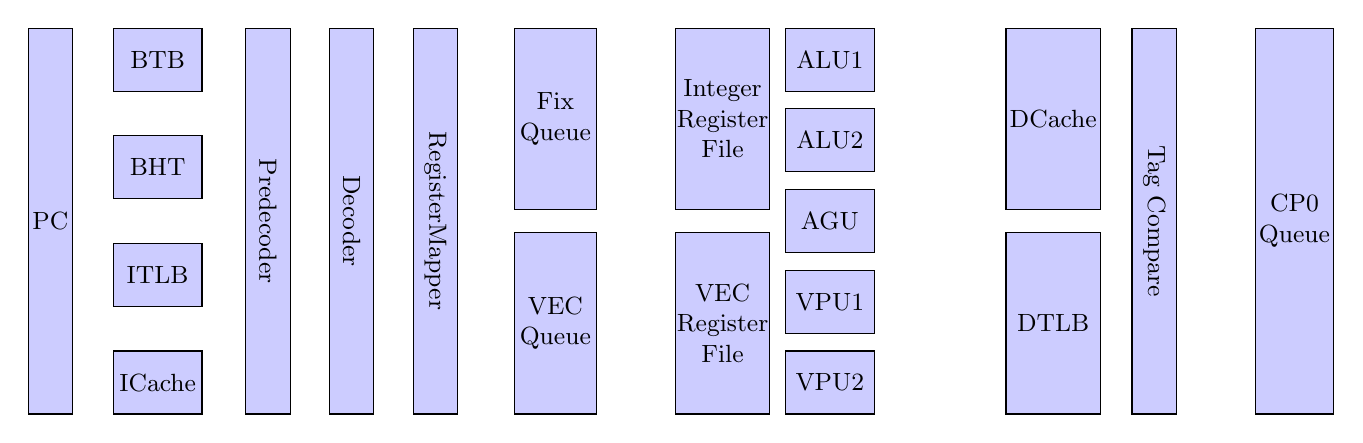
\begin{tikzpicture}

\node[lblock](PC){PC};
\coordinate  (PC1) at ($(PC.north)-(0,\sh/2)$);
\coordinate  (PC4) at ($(PC.south)+(0,\sh/2)$);
\coordinate  (PC2) at ($(PC1)!0.333!(PC4)$);
\coordinate  (PC3) at ($(PC1)!0.666!(PC4)$);

\node[sblock, right=0.8cm of PC1](BTB){BTB};
\node[sblock, right=0.8cm of PC2](BHT){BHT};
\node[sblock, right=0.8cm of PC3](ITLB){ITLB};
\node[sblock, right=0.8cm of PC4](ICache){ICache};

\node[lblock,right=2.2cm of PC](Predecoder){\rotatebox{-90}{Predecoder}};
\node[lblock,right=0.5cm of Predecoder](Decoder){\rotatebox{-90}{Decoder}};
\node[lblock,right=0.5cm of Decoder](RegisterMapper){\rotatebox{-90}{RegisterMapper}};

\coordinate  (RM1) at ($(RegisterMapper.north)-(0,\mh/2)$);
\coordinate  (RM2) at ($(RegisterMapper.south)+(0,\mh/2)$);
\node[mblock, right=1cm of RM1,  text width=1cm](FixQ){Fix Queue};
\node[mblock, right=1cm of RM2,  text width=1cm](VecQ){VEC Queue};
\node[mblock, right=1cm of FixQ, text width=1.2cm](IRF){Integer Register File};
\node[mblock, right=1cm of VecQ, text width=1.2cm](VRF){VEC Register File};

\coordinate  (RF1) at ($(IRF.north)-(0,\sh/2)$);
\coordinate  (RF5) at ($(VRF.south)+(0,\sh/2)$);
\coordinate  (RF2) at ($(RF1)!0.25!(RF5)$);
\coordinate  (RF3) at ($(RF1)!0.50!(RF5)$);
\coordinate  (RF4) at ($(RF1)!0.75!(RF5)$);
\node[sblock, right=0.8cm of RF1](ALU1){ALU1};
\node[sblock, right=0.8cm of RF2](ALU2){ALU2};
\node[sblock, right=0.8cm of RF3](AGU) {AGU};
\node[sblock, right=0.8cm of RF4](VPU1){VPU1};
\node[sblock, right=0.8cm of RF5](VPU1){VPU2};

\node[mblock, right=3cm of IRF, text width=1.2cm](DCache){DCache};
\node[mblock, right=3cm of VRF, text width=1.2cm](DTLB){DTLB};
\coordinate (DD) at ($(DCache.south)!0.5!(DTLB.north)$);

\node[lblock,right=of DD](TagCompare){\rotatebox{-90}{Tag Compare}};
\node[lblock,right=of TagCompare,text width=1cm](CP0Queue){CP0 Queue};

\end{tikzpicture}
\end{document}
